% 第 17 题多面体 ABCDEF：按固定源 PDF 矢量路径端点换算（1 pt → 0.03515 cm；斜二测画法，
% x 水平实长、y 45° 半长、z 竖直实长）。以 B 为原点。
% 实线 7 条：EC、EF、FC、FA、FD、AD、DC；虚线 8 条：BE、EG（辅助）、EA、OF、BH（辅助）、BC、AB、BO。
% G 为 AB 中点（虚线连 E）；H 在 AF 上 AH:HF=2:3（虚线连 B）。先画虚线后画实线。
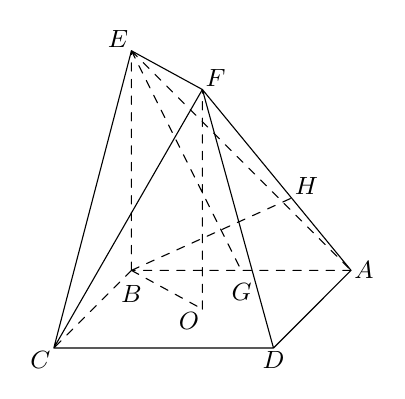
\begin{tikzpicture}[line cap=round,line join=round,font=\small]
\coordinate (B) at (0,0);
\coordinate (A) at (2.789,0);
\coordinate (C) at (-0.986,-0.986);
\coordinate (D) at (1.804,-0.986);
\coordinate (O) at (0.901,-0.492);
\coordinate (E) at (0,2.789);
\coordinate (F) at (0.901,2.297);
\coordinate (G) at (1.394,0);
\coordinate (H) at (2.034,0.919);
% 虚线先画
\draw[dashed] (B)--(E) (E)--(G) (E)--(A) (O)--(F) (B)--(H) (B)--(C) (A)--(B) (B)--(O);
% 实线后画
\draw (E)--(C) (E)--(F) (F)--(C) (F)--(A) (F)--(D) (A)--(D) (D)--(C);
\node[above left,inner sep=1pt] at (E) {$E$};
\node[above right,inner sep=1pt] at (F) {$F$};
\node[above right,inner sep=1pt] at (H) {$H$};
\node[right,inner sep=1pt] at (A) {$A$};
\node at (0,-0.30) {$B$};
\node at (1.399,-0.278) {$G$};
\node[below left,inner sep=1pt] at (O) {$O$};
\node[below left,inner sep=1pt] at (C) {$C$};
\node[below,inner sep=1pt] at (D) {$D$};
\end{tikzpicture}
